\documentclass[a4paper]{article}
\usepackage{tikz}
\usepackage{algorithm}[boxed]
\usepackage{algorithmic}
\usetikzlibrary{petri,automata,matrix,backgrounds}

\title{Converting Concurrent DFAs to a Single Petri Net}
\author{Andrew Matthews}
\begin{document}
\maketitle

In the Petri Net literature, it is not uncommon to see DFAs such as in Fig.
\ref{fig:dfa1} replaced by PTs such as in Fig. \ref{fig:ptnet1}.

\begin{figure}[ht]
	\begin{center}
		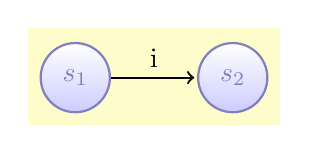
\begin{tikzpicture}[
			original state/.style={blue!50!black!50,top color=white,bottom color=blue!20},
			background rectangle/.style={fill=yellow!20}, framed,show
			background rectangle,shorten >=1pt,node distance=2cm,auto,thick]
			\node[state, original state] (q_0) {$s_1$};
			\node[state, original state] (q_1) [right of=q_0] {$s_2$};
			\path[->] (q_0) edge node [above] {i} (q_1);
		\end{tikzpicture}
	\end{center}
	\caption{A Single transition between states in a DFA}
	\label{fig:dfa1}
\end{figure}

\begin{figure}[ht]
	\begin{center}
		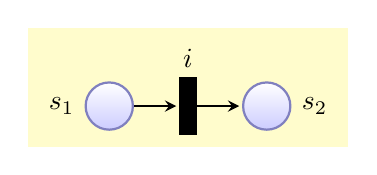
\begin{tikzpicture} [background rectangle/.style={fill=yellow!20}, framed,show
			background rectangle,yscale=1,thin,>=stealth,thick,
			original state/.style={blue!50!black!50,top color=white,bottom color=blue!20},
			input state/.style={red!50!black!50,top color=white,bottom color=red!20},
		every transition/.style={fill,minimum width=2mm,minimum height=7mm},
		every place/.style={draw,thick,minimum size=6mm}]

		\node [place, label=left:$s_1$, original state] (s_1) at (0,0) {};
		\node [place, label=right:$s_2$, original state] (s_2) at (2,0) {};
		\node [transition, label=above:$i$] (tran) at (1,0) {}
			edge [pre] (s_1)
			edge [post] (s_2);
		\end{tikzpicture}
	\end{center}
	\caption{A naive replacement of the DFA transition with a petri net
	transition}
	\label{fig:ptnet1}
\end{figure}


\begin{figure}[ht]
	\begin{center}
		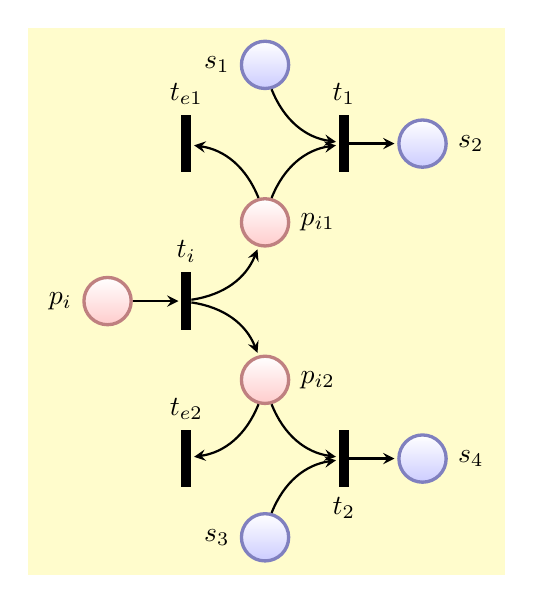
\begin{tikzpicture} [background rectangle/.style={fill=yellow!20}, framed,show
			background rectangle,yscale=1,thin,>=stealth,thick,
			every transition/.style={fill,minimum width=1mm,minimum height=7mm},
			original state/.style={blue!50!black!50,top color=white,bottom color=blue!20},
			input state/.style={red!50!black!50,top color=white,bottom color=red!20},
			every place/.style={draw,very thick,minimum size=6mm}
			]

		\node [place, original state, label=left:$s_1$] (s1) at (3,7) {};
		\node [place, input state, label=right:$p_{i1}$] (pi1) at (3,5) {};
		\node [place, original state, label=right:$s_2$] (s2) at (5,6) {};
		\node [place, input state, label=left:$p_i$] (pi) at (1,4) {};
		\node [place, input state, label=right:$p_{i2}$] (pi2) at (3,3) {};
		\node [place, original state, label=left:$s_3$] (s3) at (3,1) {};
		\node [place, original state, label=right:$s_4$] (s4) at (5,2) {};

		\node [transition, label=above:$t_{e1}$] (te1) at (2,6) {}
			edge [pre, bend left] (pi1);
		\node [transition, label=above:$t_1$] (t1) at (4,6) {}
			edge [pre, bend left] (s1)
			edge [pre, bend right] (pi1)
			edge [post] (s2);
		\node [transition, label=above:$t_i$] (ti) at (2,4) {}
			edge [pre] (pi)
			edge [post, bend right] (pi1)
			edge [post, bend left] (pi2);
		\node [transition, label=above:$t_{e2}$] (te2) at (2,2) {}
			edge [pre, bend right] (pi2);
		\node [transition, label=below:$t_2$] (t2) at (4,2) {}
			edge [pre, bend right] (s3)
			edge [pre, bend left] (pi2)
			edge [post] (s4);

		\end{tikzpicture}
	\end{center}
	\caption{A petri net that reproduces the semantics of Fig. \ref{fig:dfa1} while
	consuming unused tokens}
	\label{fig:ptnetfinal}
\end{figure}

\begin{figure}[ht]
	\begin{center}
		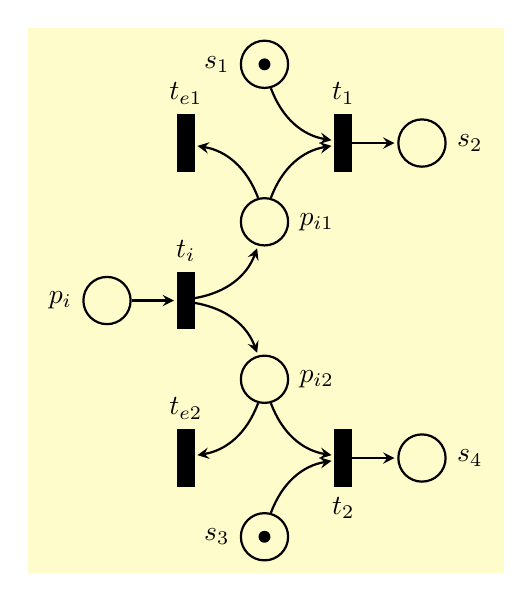
\begin{tikzpicture} [background rectangle/.style={fill=yellow!20}, framed,show
			background rectangle,yscale=1,thin,>=stealth,thick,
			every transition/.style={fill,minimum width=2mm,minimum height=7mm},
			every place/.style={draw,thick,minimum size=6mm},
			original state/.style={blue!50!black!50,top color=white,bottom color=blue!20},
			input state/.style={red!50!black!50,top color=white,bottom color=red!20}]

		\node [place, tokens=1, label=left:$s_1$] (s1) at (3,7) {};
		\node [place, label=right:$p_{i1}$] (pi1) at (3,5) {};
		\node [place, label=right:$s_2$] (s2) at (5,6) {};
		\node [place, label=left:$p_i$] (pi) at (1,4) {};
		\node [place, label=right:$p_{i2}$] (pi2) at (3,3) {};
		\node [place, tokens=1, label=left:$s_3$] (s3) at (3,1) {};
		\node [place, label=right:$s_4$] (s4) at (5,2) {};

		\node [transition, label=above:$t_{e1}$] (te1) at (2,6) {}
			edge [pre, bend left] (pi1);
		\node [transition, label=above:$t_1$] (t1) at (4,6) {}
			edge [pre, bend left] (s1)
			edge [pre, bend right] (pi1)
			edge [post] (s2);
		\node [transition, label=above:$t_i$] (ti) at (2,4) {}
			edge [pre] (pi)
			edge [post, bend right] (pi1)
			edge [post, bend left] (pi2);
		\node [transition, label=above:$t_{e2}$] (te2) at (2,2) {}
			edge [pre, bend right] (pi2);
		\node [transition, label=below:$t_2$] (t2) at (4,2) {}
			edge [pre, bend right] (s3)
			edge [pre, bend left] (pi2)
			edge [post] (s4);

		\end{tikzpicture}
	\end{center}
	\caption{A petri net that reproduces the semantics of Fig. \ref{fig:dfa1} while
	consuming unused tokens}
	\label{fig:ptnetfinal}
\end{figure}


\begin{figure}[ht]
	\begin{center}
		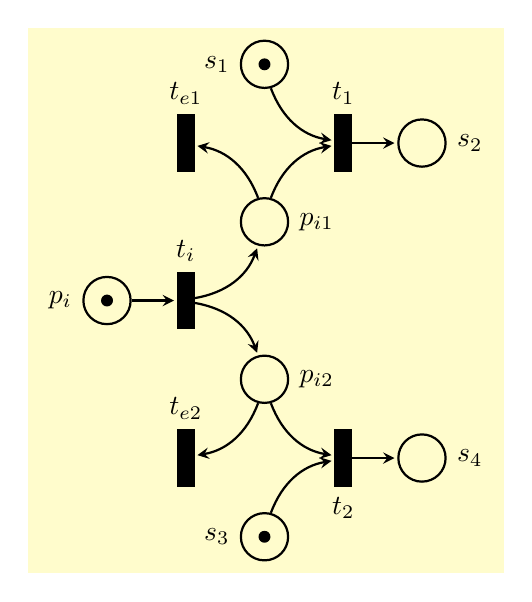
\begin{tikzpicture} [background rectangle/.style={fill=yellow!20}, framed,show
			background rectangle,yscale=1,thin,>=stealth,thick,
			every transition/.style={fill,minimum width=2mm,minimum height=7mm},
			original state/.style={blue!50!black!50,top color=white,bottom color=blue!20},
			input state/.style={red!50!black!50,top color=white,bottom color=red!20},
			every place/.style={draw,thick,minimum size=6mm}]

		\node [place, tokens=1, label=left:$s_1$] (s1) at (3,7) {};
		\node [place, label=right:$p_{i1}$] (pi1) at (3,5) {};
		\node [place, label=right:$s_2$] (s2) at (5,6) {};
		\node [place, tokens=1, label=left:$p_i$] (pi) at (1,4) {};
		\node [place, label=right:$p_{i2}$] (pi2) at (3,3) {};
		\node [place, tokens=1, label=left:$s_3$] (s3) at (3,1) {};
		\node [place, label=right:$s_4$] (s4) at (5,2) {};

		\node [transition, label=above:$t_{e1}$] (te1) at (2,6) {}
			edge [pre, bend left] (pi1);
		\node [transition, label=above:$t_1$] (t1) at (4,6) {}
			edge [pre, bend left] (s1)
			edge [pre, bend right] (pi1)
			edge [post] (s2);
		\node [transition, label=above:$t_i$] (ti) at (2,4) {}
			edge [pre] (pi)
			edge [post, bend right] (pi1)
			edge [post, bend left] (pi2);
		\node [transition, label=above:$t_{e2}$] (te2) at (2,2) {}
			edge [pre, bend right] (pi2);
		\node [transition, label=below:$t_2$] (t2) at (4,2) {}
			edge [pre, bend right] (s3)
			edge [pre, bend left] (pi2)
			edge [post] (s4);

		\end{tikzpicture}
	\end{center}
	\caption{A petri net that reproduces the semantics of Fig. \ref{fig:dfa1} while
	consuming unused tokens}
	\label{fig:ptnetfinal}
\end{figure}


\begin{figure}[ht]
	\begin{center}
		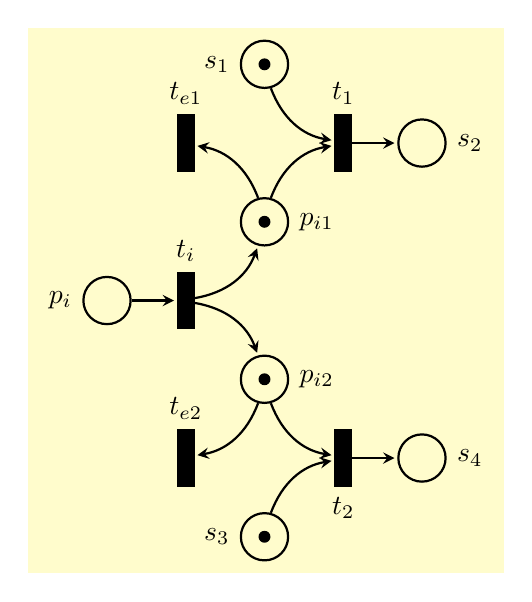
\begin{tikzpicture} [background rectangle/.style={fill=yellow!20}, framed,show
			background rectangle,yscale=1,thin,>=stealth,thick,
			every transition/.style={fill,minimum width=2mm,minimum height=7mm},
			original state/.style={blue!50!black!50,top color=white,bottom color=blue!20},
			input state/.style={red!50!black!50,top color=white,bottom color=red!20},
			every place/.style={draw,thick,minimum size=6mm}]

		\node [place, tokens=1, label=left:$s_1$] (s1) at (3,7) {};
		\node [place, tokens=1, label=right:$p_{i1}$] (pi1) at (3,5) {};
		\node [place, label=right:$s_2$] (s2) at (5,6) {};
		\node [place, tokens=0, label=left:$p_i$] (pi) at (1,4) {};
		\node [place, tokens=1, label=right:$p_{i2}$] (pi2) at (3,3) {};
		\node [place, tokens=1, label=left:$s_3$] (s3) at (3,1) {};
		\node [place, label=right:$s_4$] (s4) at (5,2) {};

		\node [transition, label=above:$t_{e1}$] (te1) at (2,6) {}
			edge [pre, bend left] (pi1);
		\node [transition, label=above:$t_1$] (t1) at (4,6) {}
			edge [pre, bend left] (s1)
			edge [pre, bend right] (pi1)
			edge [post] (s2);
		\node [transition, label=above:$t_i$] (ti) at (2,4) {}
			edge [pre] (pi)
			edge [post, bend right] (pi1)
			edge [post, bend left] (pi2);
		\node [transition, label=above:$t_{e2}$] (te2) at (2,2) {}
			edge [pre, bend right] (pi2);
		\node [transition, label=below:$t_2$] (t2) at (4,2) {}
			edge [pre, bend right] (s3)
			edge [pre, bend left] (pi2)
			edge [post] (s4);

		\end{tikzpicture}
	\end{center}
	\caption{A petri net that reproduces the semantics of Fig. \ref{fig:dfa1} while
	consuming unused tokens}
	\label{fig:ptnetfinal}
\end{figure}


\begin{figure}[ht]
	\begin{center}
		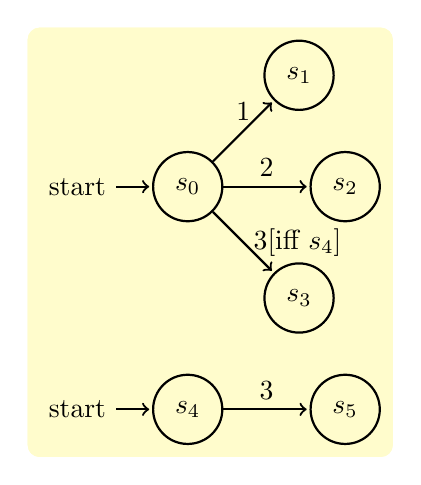
\begin{tikzpicture} [
			original state/.style={blue!50!black!50,top color=white,bottom color=blue!20},
			input state/.style={red!50!black!50,top color=white,bottom color=red!20},
		  background rectangle/.style={fill=yellow!20}, framed,show
			background rectangle,rounded corners=1ex,shorten >=1pt,node distance=2cm,auto,thick]
			\node[state,initial] (s_0) {$s_0$};
			\node[state] (s_1) [above right of=s_0] {$s_1$};
			\node[state] (s_2) [right of=s_0]{$s_2$};
			\node[state] (s_3) [below right of=s_0]{$s_3$};
			\path[->] (s_0) edge node [above] {1} (s_1);
			\path[->] (s_0) edge node [above] {2} (s_2);
			\path[->] (s_0) edge node [right] {3[iff $s_4$]} (s_3);

			\node[state,initial] (s_4) [below left of=s_3]{$s_4$};
			\node[state] (s_5) [right of=s_4]{$s_5$};
			\path[->] (s_4) edge node [above] {3} (s_5);
		\end{tikzpicture}
	\end{center}

	\caption{The original problem}
	\label{fig:originalProblem}
\end{figure}

I initially thought that I could proceed easily with the existing model with
only minor modifications. After a little thought and exploration, it 
became clear that there were more efficiencies and greater expressive power to
be gained from changing the way that the state models were represented.

The first thing that I thought was that 13 DFAs is really only a
single NDFA with 13 disconnected subgraphs. I wondered whether by merging the
graphs into a combined graph with merged states, I might be able to transmute
the existing state transitions into new ones where the illegal state transitions
were just not possible. It quickly became clear that that was just not feasible.
It's not too difficult to do the conversion, but representing the resulting
graph in any form that us humans could interpret would be impossible. As an
intermediate representation it might be useful, so I didn't rule it out.

My next thought was that the state machine could still be converted into a
NDFA, but that we didn't necessarily need to merge the state models. We could
decree that they were all part of one DFA and that they were just coincidentally
deterministic. After all, a deterministic state machine is just a special sort of
nondeterministic one!

Having done that, I figured I could somehow wire up the state machines to allow
them to veto the transitions made by other state models. At that point, I
started to think that a Petri Net was my best way to control the transitions in
the state models so that they carried on behaving like deterministic automata,
even though they partook of nondeterminism in an intermediate state.

\begin{algorithm}
\caption{Constructing a Petri Net Adjacency Matrix for a DFA}
\label{alg1}
	
\begin{algorithmic}
	\REQUIRE an adjacency list $A$
	\REQUIRE a \verb|DFA| $D = <S, \delta, \Sigma, i>$
	\STATE Create places $e$, $p_z$ in $A$
	\STATE Carry out some processing
	\STATE Create a single place $e$ (the exhaust trigger place)
	\STATE Create a single place $p_z$ (the exhaust sink)

	\FORALL{inputs $i$ in $\Sigma$}
		\STATE create transition $t_{s_i}$ in $A$ (the input sink transition for $p_i$) adjacent to $p_z$
		\STATE create place $p_i$ in $A$ adjacent to $t_{s_i}$
		\STATE mark $e$ as adjacent to $t_{s_i}$ 
		\STATE mark $p_i$ as adjacent to $t_{s_i}$ 
	\ENDFOR

	\FORALL{states $s$ in $S$}
		\STATE create a place $p_s$ in $A$
	\ENDFOR

	\FORALL{$t = (s_1, s_2, i)$ in $\delta$}
		\STATE Create a new transition $t_{s_1 i s_2}$ in $A$
		\STATE Mark place $p_{s_1}$ (where $s_1$ was defined earlier) adjacent to  $t_{(s_1, s_2, i)}$
		\STATE Mark place  $t_{(s_1, s_2, i)}$ adjacent to  $p_{s_2}$
	\ENDFOR
\end{algorithmic}
\end{algorithm}

If we use an adjacency list representation to encode the information set above
we will add the adjacencies in \ref{fig:adjList1} for each edge in $D$.

\begin{figure}[ht]
	\begin{center}
		\begin{displaymath}
		\begin{array}{lll}
			e & \to  & t_{s_i} \\
			p_i & \to  & t_{s_i}, t_{(s_1, s_2, i)} \\
			s_1 & \to  & t_{(s_1, s_2, i)} \\
			t_{s_i} &\to & p_z \\
			t_{(s_1, s_2, i)} & \to  & s_2 \\
		\end{array}
		\end{displaymath}
	\end{center}
	\caption{An adjacency list avoids the waste of a sparse matrix}
	\label{fig:adjList1}
\end{figure}

For the sake of clarity, let's look at an adjacency matrix representation of the
same imformation. For most DFAs the matrix will be sparse so it would not make
much sense to use a matrix in practice, but for this exploration we can use one
to see what the result will be.

\subsection{ Space requirements }

Given a Deterministic Finite Automaton $D \equiv S \times \delta \times \Sigma
\times i$

For every input symbol $i$ in $\Sigma$ we require a place ($p_i$) to allow
signalling of input of that input type, an exhaust (or sink) transition
($t_{s_i}$) allowing removal of input marks after an input cycle and one arc
between the place and the transition. Each original arc in the DFA is now
replaced by two arcs and a transition.

Assuming that we use integers to represent both states and inputs, an adjacency
list representation will contain both predictable infrastructure wiring as well
as DFA sepecific overheads.

\[
C = 2(|\Sigma|) + 3(|\delta|) + |\delta| + |\Sigma|
\]

So, for a DFA with 69 states, 358 transitions and 121 unique inputs the
additional cost is \[
C= (3 \times 121 + 4 \times 358) \times 4
=1795 \times 4
=7.2\mathrm{KB}
\]

By contrast the object graph representation used in AgentDesktop consumes 20
bytes per state and 24 bytes per transition yielding a total cost of 9.9K


A transition has no specific triggers other than the presence of a token in all
of its input places. The transition will fire if ever the input place gets a
mark. We need it to be triggered only in the presence of the input. To do that
with a petri net, we add a single pllace for each possible input.

\begin{figure}[ht]
	\begin{center}
		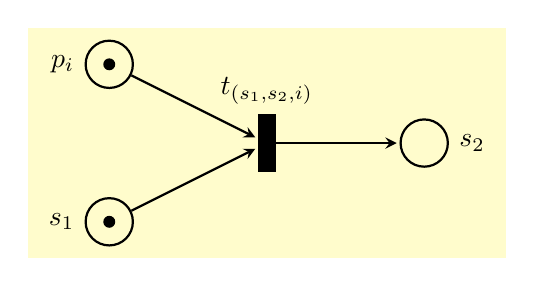
\begin{tikzpicture} [background rectangle/.style={fill=yellow!20}, framed,show
			background rectangle,yscale=1,thin,>=stealth,thick,
			original state/.style={blue!50!black!50,top color=white,bottom color=blue!20},
			input state/.style={red!50!black!50,top color=white,bottom color=red!20},
		every transition/.style={fill,minimum width=2mm,minimum height=7mm},
		every place/.style={draw,thick,minimum size=6mm}]

			\node [place, tokens=1, label=left:$p_i$] (place-pi) at ( 0,3) {};
			\node [place, tokens=1, label=left:$s_1$] (place-v1) at ( 0,1) {};
			\node [place, label=right:$s_2$] (place-v2) at ( 4,2) {};

			\node [transition, label=above:$t_{(s_1, s_2, i)}$] (tran-ti) at ( 2,2) {}
				edge [pre] (place-v1)
				edge [pre] (place-pi)
				edge [post](place-v2);
		\end{tikzpicture}
	\end{center}
	\caption{A less naive petri net that fires only when the place for a certain
	input is is marked.}
	\label{fig:ptnet3}
\end{figure}

A petri net is designed to retain the marking for a state indefinitely, if it is
not consumed. The diagram above deviate

\begin{figure}[ht]
	\begin{center}
		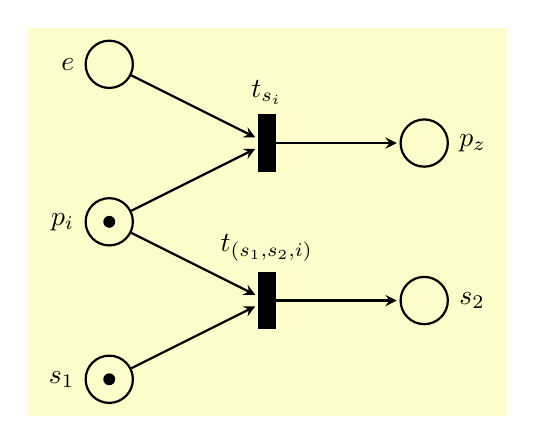
\begin{tikzpicture} [background rectangle/.style={fill=yellow!20}, framed,show
			background rectangle,yscale=1,thin,>=stealth,thick,
			original state/.style={blue!50!black!50,top color=white,bottom color=blue!20},
			input state/.style={red!50!black!50,top color=white,bottom color=red!20},
		every transition/.style={fill,minimum width=2mm,minimum height=7mm},
		every place/.style={draw,thick,minimum size=6mm}]

			\node [place, label=left:$e$] (place-e) at ( 0,5) {};
			\node [place, tokens=1, label=left:$p_i$] (place-pi) at ( 0,3) {};
			\node [place, tokens=1, label=left:$s_1$] (place-v1) at ( 0,1) {};
			\node [place, label=right:$p_z$] (place-pz) at ( 4,4) {};
			\node [place, label=right:$s_2$] (place-v2) at ( 4,2) {};

			\node [transition, label=above:$t_{s_i}$] (tran-ts) at ( 2,4) {}
				edge [pre] (place-e)
				edge [pre] (place-pi)
				edge [post] (place-pz);
			\node [transition, label=above:$t_{(s_1, s_2, i)}$] (tran-ti) at ( 2,2) {}
				edge [pre] (place-v1)
				edge [pre] (place-pi)
				edge [post](place-v2);
		\end{tikzpicture}
	\end{center}
	\caption{A petri net that reproduces the semantics of Fig. \ref{fig:dfa1} while
	consuming unused tokens}
	\label{fig:ptnet2}
\end{figure}

\begin{figure}[ht]
	\begin{center}
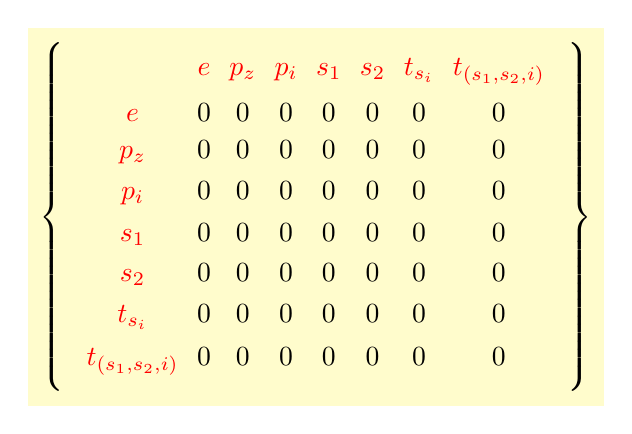
\begin{tikzpicture}[background rectangle/.style={fill=yellow!20}, framed,show
			background rectangle,column 1/.style=red, row 1/.style=red]
\matrix [matrix of math nodes,left delimiter=\{,right delimiter=\}]
{
& e & p_z & p_i & s_1 & s_2 & t_{s_i} & t_{(s_1, s_2, i)} \\
e   & 0 & 0 & 0 & 0 & 0 & 0 & 0 \\
p_z & 0 & 0 & 0 & 0 & 0 & 0 & 0 \\
p_i & 0 & 0 & 0 & 0 & 0 & 0 & 0 \\
s_1 & 0 & 0 & 0 & 0 & 0 & 0 & 0 \\
s_2 & 0 & 0 & 0 & 0 & 0 & 0 & 0 \\
t_{s_i} & 0 & 0 & 0 & 0 & 0 & 0 & 0 \\
t_{(s_1, s_2, i)} & 0 & 0 & 0 & 0 & 0 & 0 & 0 \\
};
\end{tikzpicture}
	\end{center}
	\caption{An adjacency matrix with no arcs set}
	\label{fig:adjMatrix1}
\end{figure}

\begin{figure}[ht]
	\begin{center}
		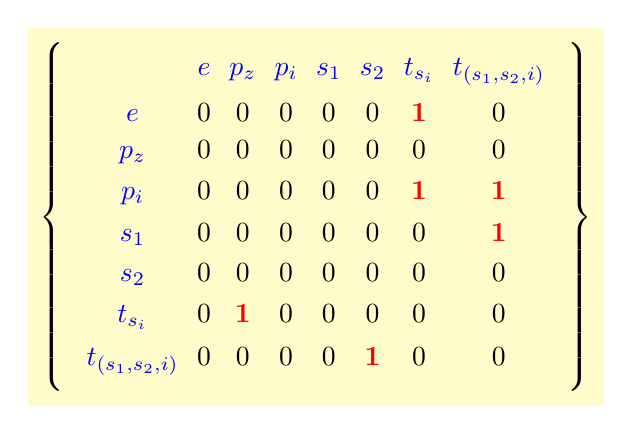
\begin{tikzpicture}[background rectangle/.style={fill=yellow!20}, framed,show
			background rectangle,column 1/.style=blue, row 1/.style=blue]
		\matrix [matrix of math nodes,left delimiter=\{,right delimiter=\}]
		{
		& e & p_z & p_i & s_1 & s_2 & t_{s_i} & t_{(s_1, s_2, i)} \\
		e   & 0 & 0 & 0 & 0 & 0 & |[red]|\textbf{1} & 0 \\
		p_z & 0 & 0 & 0 & 0 & 0 & 0 & 0 \\
		p_i & 0 & 0 & 0 & 0 & 0 & |[red]| \textbf{1} & |[red]| \textbf{1} \\
		s_1 & 0 & 0 & 0 & 0 & 0 & 0 & |[red]| \textbf{1} \\
		s_2 & 0 & 0 & 0 & 0 & 0 & 0 & 0 \\
		t_{s_i} & 0 & |[red]| \textbf{1} & 0 & 0 & 0 & 0 & 0 \\
		t_{(s_1, s_2, i)} & 0 & 0 & 0 & 0 & |[red]| \textbf{1} & 0 & 0 \\
		};
		\end{tikzpicture}
	\end{center}
	\caption{The Adjacency matrix with the arcs for Fig. \ref{fig:ptnet2} added}
	\label{fig:adjMatrix2}
\end{figure}
\end{document}



